\documentclass{article}
\usepackage[T1]{fontenc}
\usepackage{lmodern}
\usepackage{graphicx}
\usepackage{amsmath,amssymb}
\usepackage[a4paper,margin=2cm]{geometry}
\usepackage[absolute,overlay]{textpos}
\setlength{\TPHorizModule}{1mm}
\setlength{\TPVertModule}{1mm}
\usepackage[indonesian]{babel}
\usepackage{hyperref}
\setlength{\emergencystretch}{2em}
% unit: Halaman 34

\begin{document}

% === Halaman 34 (llm) ===

\vspace{147.01mm}

Cover image
\vspace{20mm}
Embedded image

\vspace{111.67mm}

% deskripsi: Gambar seekor hewan berwarna putih di atas salju yang digunakan sebagai contoh 'Cover image'.
% bbox normalisasi: [0.1520, 0.0260, 0.5550, 0.5210]
\begin{textblock*}{84.63mm}(31.92mm,7.72mm)
\noindent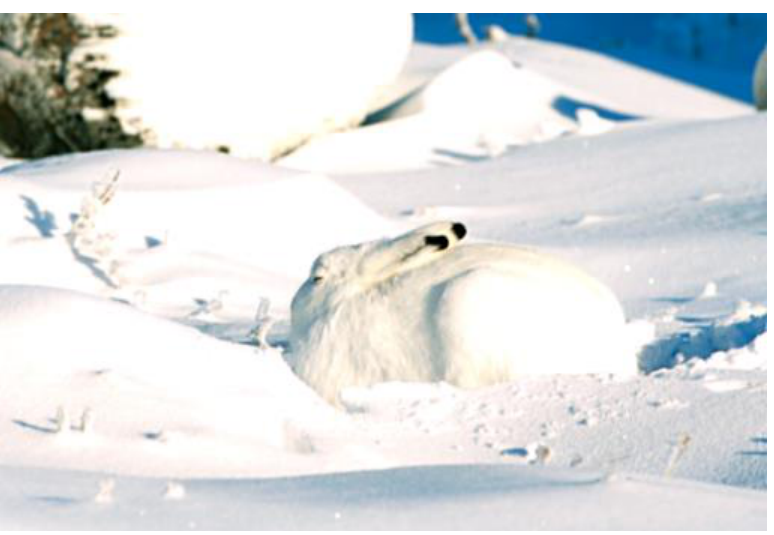
\includegraphics[width=84.63mm,height=147.01mm]{../../images/llm/page_034_img_01.png}%
\end{textblock*}

% deskripsi: Gambar sebuah pesawat jet tempur yang digunakan sebagai contoh 'Embedded image'.
% bbox normalisasi: [0.5190, 0.5280, 0.8330, 0.9040]
\begin{textblock*}{65.94mm}(108.99mm,156.82mm)
\noindent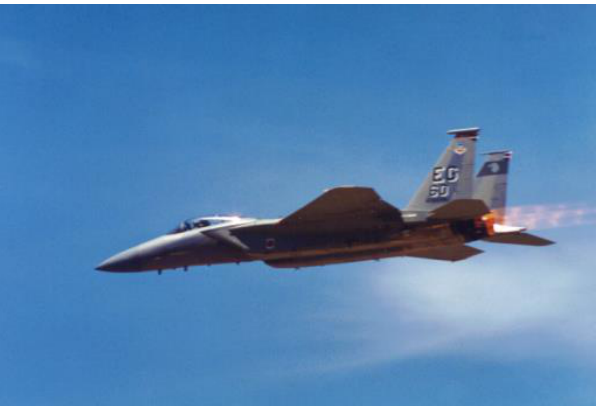
\includegraphics[width=65.94mm,height=111.67mm]{../../images/llm/page_034_img_02.png}%
\end{textblock*}

\end{document}
